\documentclass[a4paper,UKenglish]{oasics-v2016}
%This is a template for producing OASIcs articles. 
%See oasics-v2016-manual.pdf for further information.
%for A4 paper format use option "a4paper", for US-letter use option "letterpaper"
%for british hyphenation rules use option "UKenglish", for american hyphenation rules use option "USenglish"
% for section-numbered lemmas etc., use "numberwithinsect"
 
\usepackage{microtype}%if unwanted, comment out or use option "draft"
\usepackage{graphicx}
\graphicspath{ {Plots/} }

%\graphicspath{{./graphics/}}%helpful if your graphic files are in another directory

\bibliographystyle{plainurl}% the recommended bibstyle

% Author macros::begin %%%%%%%%%%%%%%%%%%%%%%%%%%%%%%%%%%%%%%%%%%%%%%%%
\title{Discriminative and Generative models for clinical risk estimation: An empirical comparison}
\titlerunning{Discriminative and Generative models for clinical risk estimation: An empirical comparison} %optional, in case that the title is too long; the running title should fit into the top page column

%% Please provide for each author the \author and \affil macro, even when authors have the same affiliation, i.e. for each author there needs to be the  \author and \affil macros
\author[1]{John Stamford}
\author[2]{Chandra Kambhampati}
\affil[1]{Department of Computer Science, The University of Hull, Kingston upon Hull, HU6 7RX\\
\texttt{j.stamford@2014.hull.ac.uk}}
\affil[2]{Department of Computer Science, The University of Hull, Kingston upon Hull, HU6 7RX\\
\texttt{c.kambhampati@hull.ac.uk}}


\authorrunning{John Stamford, Chandra Kambhampati} %mandatory. First: Use abbreviated first/middle names. Second (only in severe cases): Use first author plus 'et. al.'

\Copyright{John Stamford}%mandatory, please use full first names. OASIcs license is "CC-BY";  http://creativecommons.org/licenses/by/3.0/

\subjclass{ D.4.8 Performance }% mandatory: Please choose ACM 1998 classifications from http://www.acm.org/about/class/ccs98-html . E.g., cite as "F.1.1 Models of Computation". 
\keywords{Discriminative, Generative, Naïve Bayes, Logistic Regression, Clinical Risk}% mandatory: Please provide 1-5 keywords
% Author macros::end %%%%%%%%%%%%%%%%%%%%%%%%%%%%%%%%%%%%%%%%%%%%%%%%%

%Editor-only macros:: begin (do not touch as author)%%%%%%%%%%%%%%%%%%%%%%%%%%%%%%%%%%
\EventEditors{Fergus Leahy}
\EventNoEds{2}
\EventLongTitle{Discriminative and Generative models for clinical risk estimation: An empirical comparison}
\EventShortTitle{ICCSW 2017}
\EventAcronym{ICCSW}
\EventYear{2017}
\EventDate{September 26th and 27th, 2017}
\EventLocation{Imperial College London, United Kingdom}
\EventLogo{}
\SeriesVolume{42}
\ArticleNo{23}
% Editor-only macros::end %%%%%%%%%%%%%%%%%%%%%%%%%%%%%%%%%%%%%%%%%%%%%%%

\begin{document}

\maketitle

\begin{abstract}
Linear discriminative models, in the form of Logistic Regression, are a popular choice within the clinical domain in the development of risk models. Logistic regression is commonly used as it offers explanatory information in addition to its predictive capabilities. In some examples the coefficients from these models have been used to determine overly simplified clinical risk scores. Such models are constrained to modeling linear relationships between the variables and the class despite it known that this relationship is not always linear. This paper compares the conditions under which linear discriminative and linear generative models perform best. This is done through comparing logistic regression and naïve Bayes on real clinical data. The work shows that generative models perform best when the internal representation of the data is closer to the true distribution of the data and when there is a very small difference between the means of the classes. When looking at variables such as sodium it is shown that logistic regression can not model the observed risk as it is non-linear in its nature, whereas naïve Bayes gives a better estimation of risk. The work concludes that the risk estimations derived from discriminative models such as logistic regression need to be considered in the wider context of the true risk observed within the dataset.
 \end{abstract}



\section{Introduction}
Within the clinical domain the use of linear discriminative models such as logistic regression is a popular choice in the development of clinical risk models. Such models are able to model linear relationships between continuous variables and binary outcome events such as mortality. Generally discriminative models are preferred over generative models, however, there is a need to understand the conditions under which these models perform best [1]. Within the context of clinical risk modelling we aim to explore these conditions. This is achieved by selecting logistic regression as a linear discriminative model and comparing this to naïve Bayes which is as a linear generative model.

Logistic regression is a linear discriminative model which estimates probability directly from the inputs $x$ and the class label $y$. The posterior probability is estimated directly as a function of $p(y|x)$. Logistic regression is widely applied in the clinical domain and has shown to be effective for modelling clinical risk. The popularity of this approach in the clinical domain is the dual ability of the model to offer explanatory information about the underlying causes as well as its predictive capability. The main limitation of logistic regression is the estimated coefficients model linear relationships between the input variables and the class label.

To compare the differences between discriminative and generative models in the clinical context a naïve Bayes model is selected as it is a linear generative model. Naïve Bayes determines probability estimates from the joint probability expressed as $p(x,y)$. Probability estimates are derived by estimating the probability $p(y|x)$ for each class label based on the input, then using Bayes rule to determine the most likely class. Whilst naïve Bayes is considered a linear model, the probability estimates derived from the function $p(x,y)$ can model non-linear relationships between the inputs and the class label.


\section{Background}
As discussed, discriminative models are commonly applied to clinical data usually in the form of logistic regression for the use of both explanatory and predictive purposes. It is shown that logistic regression is widely used in the prediction of mortality events in addition to predicting hospital readmission, and it is able to outperform other regression techniques [2]. In other examples it is shown that logistic regression has been used to model short term mortality events including death within 30 days [3] and death within 60 days [4]. In these examples the performance was reported as area under the curve (AUC) with results of 0.86 and 0.77 respectively.

In other work, the coefficients from regression models have been used to develop simpler points based models for use in clinical practice [5][6]. The points are produced by rounding the estimated coefficients of the model to an integer value [6][7]. These integer values represent univariate risk with the sum representing a compound risk score.

Logistic regression is an extension of linear regression. With linear regression estimations been determined as
\begin{equation}
y = f(x,\beta) = \beta_0 + \beta_1 x_1, + ... +, \beta_n x_n + \varepsilon 
\end{equation}

where $\beta_n$ is some estimated coefficients and $\varepsilon$ represents the error. This is then extended to the general linear model of logistic regression where the estimates are bound to values between 0 and 1 through the use of a logistic sigmoid function such as
\begin{equation}
f(y|x,\beta) = \frac{1}{1 + e^{-(\beta_0 + \beta_1 x_1, + ... +, \beta_n x_n)}}
\end{equation}


Regression models allow the combination of discrete and continuous input variables to be used which allows for the estimation of a linear relationship. It is useful to transform some continuous variables into categorical variables using arbitrary ranges. For example, a continuous variable could be transformed into a categorical variable with ranges representing low, medium and high. This can be seen in existing clinical risk models [5][6].  Whilst this can help model nonlinear relationships between the variable and the class it can lead to unnatural step changes in risk between each category [8].

Naïve Bayes is an example of a generative linear model which has been applied to the clinical domain. In terms of accuracy, non-linear discriminative models such as Support Vector Machines and Decision Tress have performed marginally better than naïve Bayes at identifying patients at risk of having heart failure [9][10]. However when comparing naïve Bayes with a Multi-Layer Perceptron, which is a discriminative general non-linear model, naïve Bayes has performed better [10]. Naïve Bayes can be applied in different forms which is underpinned by the type of data which is required as the inputs. This can include multinomial naïve Bayes and Gaussian naïve Bayes. Recent work has shown that Tree Augmented naïve Bayes can perform better than other versions of naïve Bayes in the clinical domain [11].

As introduced previously, naïve Bayes estimates the probability from the joint probability expressed as $p(x,y)$. For each class the probability is estimated as
\begin{equation}
p(Y_1|x) = \frac {p(x|Y_1)p(Y_1)} { p(x|Y_1)p(Y_1) + p(x|Y_2)p(Y_2) }
\end{equation}

This gives a probability estimate for class 1 and when the problem is constrained to two classes the estimation for class 0 can be $p(Y_0|x) = 1 - p(Y_1|x)$.

In this work we are using a Gaussian naïve Bayes model which determines $p(Y_n|x)$ where $x \in X$ and $X$ conforms to a normal distribution. Within clinical dataset this requirement is commonly unsatisfied.  

\section{Dataset and Methodology}
The dataset used in this study is a subset which is extracted from the MIMIC-III dataset [12] where heart failure patients have been identified. Patients are selected based on the use of heart failure related ICD Codes in position one, two or three of the admission diagnosis. Additionally, patients without a test for N-terminal pro-B-type natriuretic peptide (NTproBNP) was excluded as this is a valuable marker in the diagnosis of patients with heart failure [13]. The subset used contained 2,536 patients with 90 day mortality used as the class labels (Dead: 697, Alive: 1839).

Naïve Bayes and logistic regression was used for univariate analysis of the datasets. Performance of the models is measured using the Pseudo R2, the means square error (MSE) and the area under the curve (AUC).

The aim of the work is to explore how discriminative and generative models perform using real clinical data. This is achieved by comparing the commonly applied logistic regression model with naïve Bayes which are both linear models.


\section{Results}



The results show the performance of the two models on clinical data, specifically showing the univariate relationship between the variable and risk of death within 90 days. The results also visually show the risk estimates derived from the two models (Figure \ref{fig:sodium} and \ref{fig:ntprobnp}).  Additionally, a sample range is selected from each variable with risk estimates from the models compared to the true proportion of risk in those ranges. As the outputs from the models are probabilistic estimates of risk rather than classification values the AUC is reported. R2 and MSE give representations of the distance between the probabilistic estimates and the true binary outcomes.



\subsection*{Risk Estimations}
The distributions of the MCV and Sodium variables approximate a Gaussian distribution along with similar means and standard deviations for the two classes (Table \ref{table:means} and Figure \ref{fig:sodium}). In these examples linear discrimination between the two classes is not possible. This is reflected in the probabilistic risk estimates derived from the logistic regression model which shows little change in risk as values for MCV and Sodium change. Furthermore, the risk estimations for these two variables is low and when interpreting 
the relationship between sodium or MCV and the risk of death using a logistic regression model these variables can be said to be poor predictors. However the probabilistic estimates derived from the naïve Bayes show a different relationship between these variables and risk. It is known that levels of sodium which are too high or too low can increase the risk of death [14]. From the distributions shown in Figure \ref{fig:sodium} for both MCV and Sodium it is intuitive that risk is increased for low and high values of these variables and risk is reduced in the mid ranges. As naïve Bayes derives its estimates from the mean and standard deviation of the classes it can better approximate the relationship between theses variables and outcome when the means are similar but the standard deviations are different. When considering this in terms of detecting patients at risk, the naïve Bayes would enable a larger number of patients at risk of death to be identified (increasing sensitivity) at the cost of incorrectly identifying low risk patients as high risk (decreased specificity). 


\begin{table}[h!]
\centering
\caption{Mean and standard deviation (SD) for MCV and Sodium for each class}
\label{table:means}
\begin{tabular}{lll|ll}
\hline
\textbf{}            & \multicolumn{2}{c|}{\textbf{Alive}}  & \multicolumn{2}{c}{\textbf{Dead}} \\

\textbf{Variable}        & \textbf{Mean}         & \textbf{SD}        & \textbf{Mean}         & \textbf{SD}         \\
\hline       
MCV     & 89.9        & 6.8       & 90.2        & 7.1       \\
Sodium  & 138.4        & 4.7       & 138.4        & 5.9       \\
\hline
\end{tabular}
\end{table}


\begin{figure}[h!]
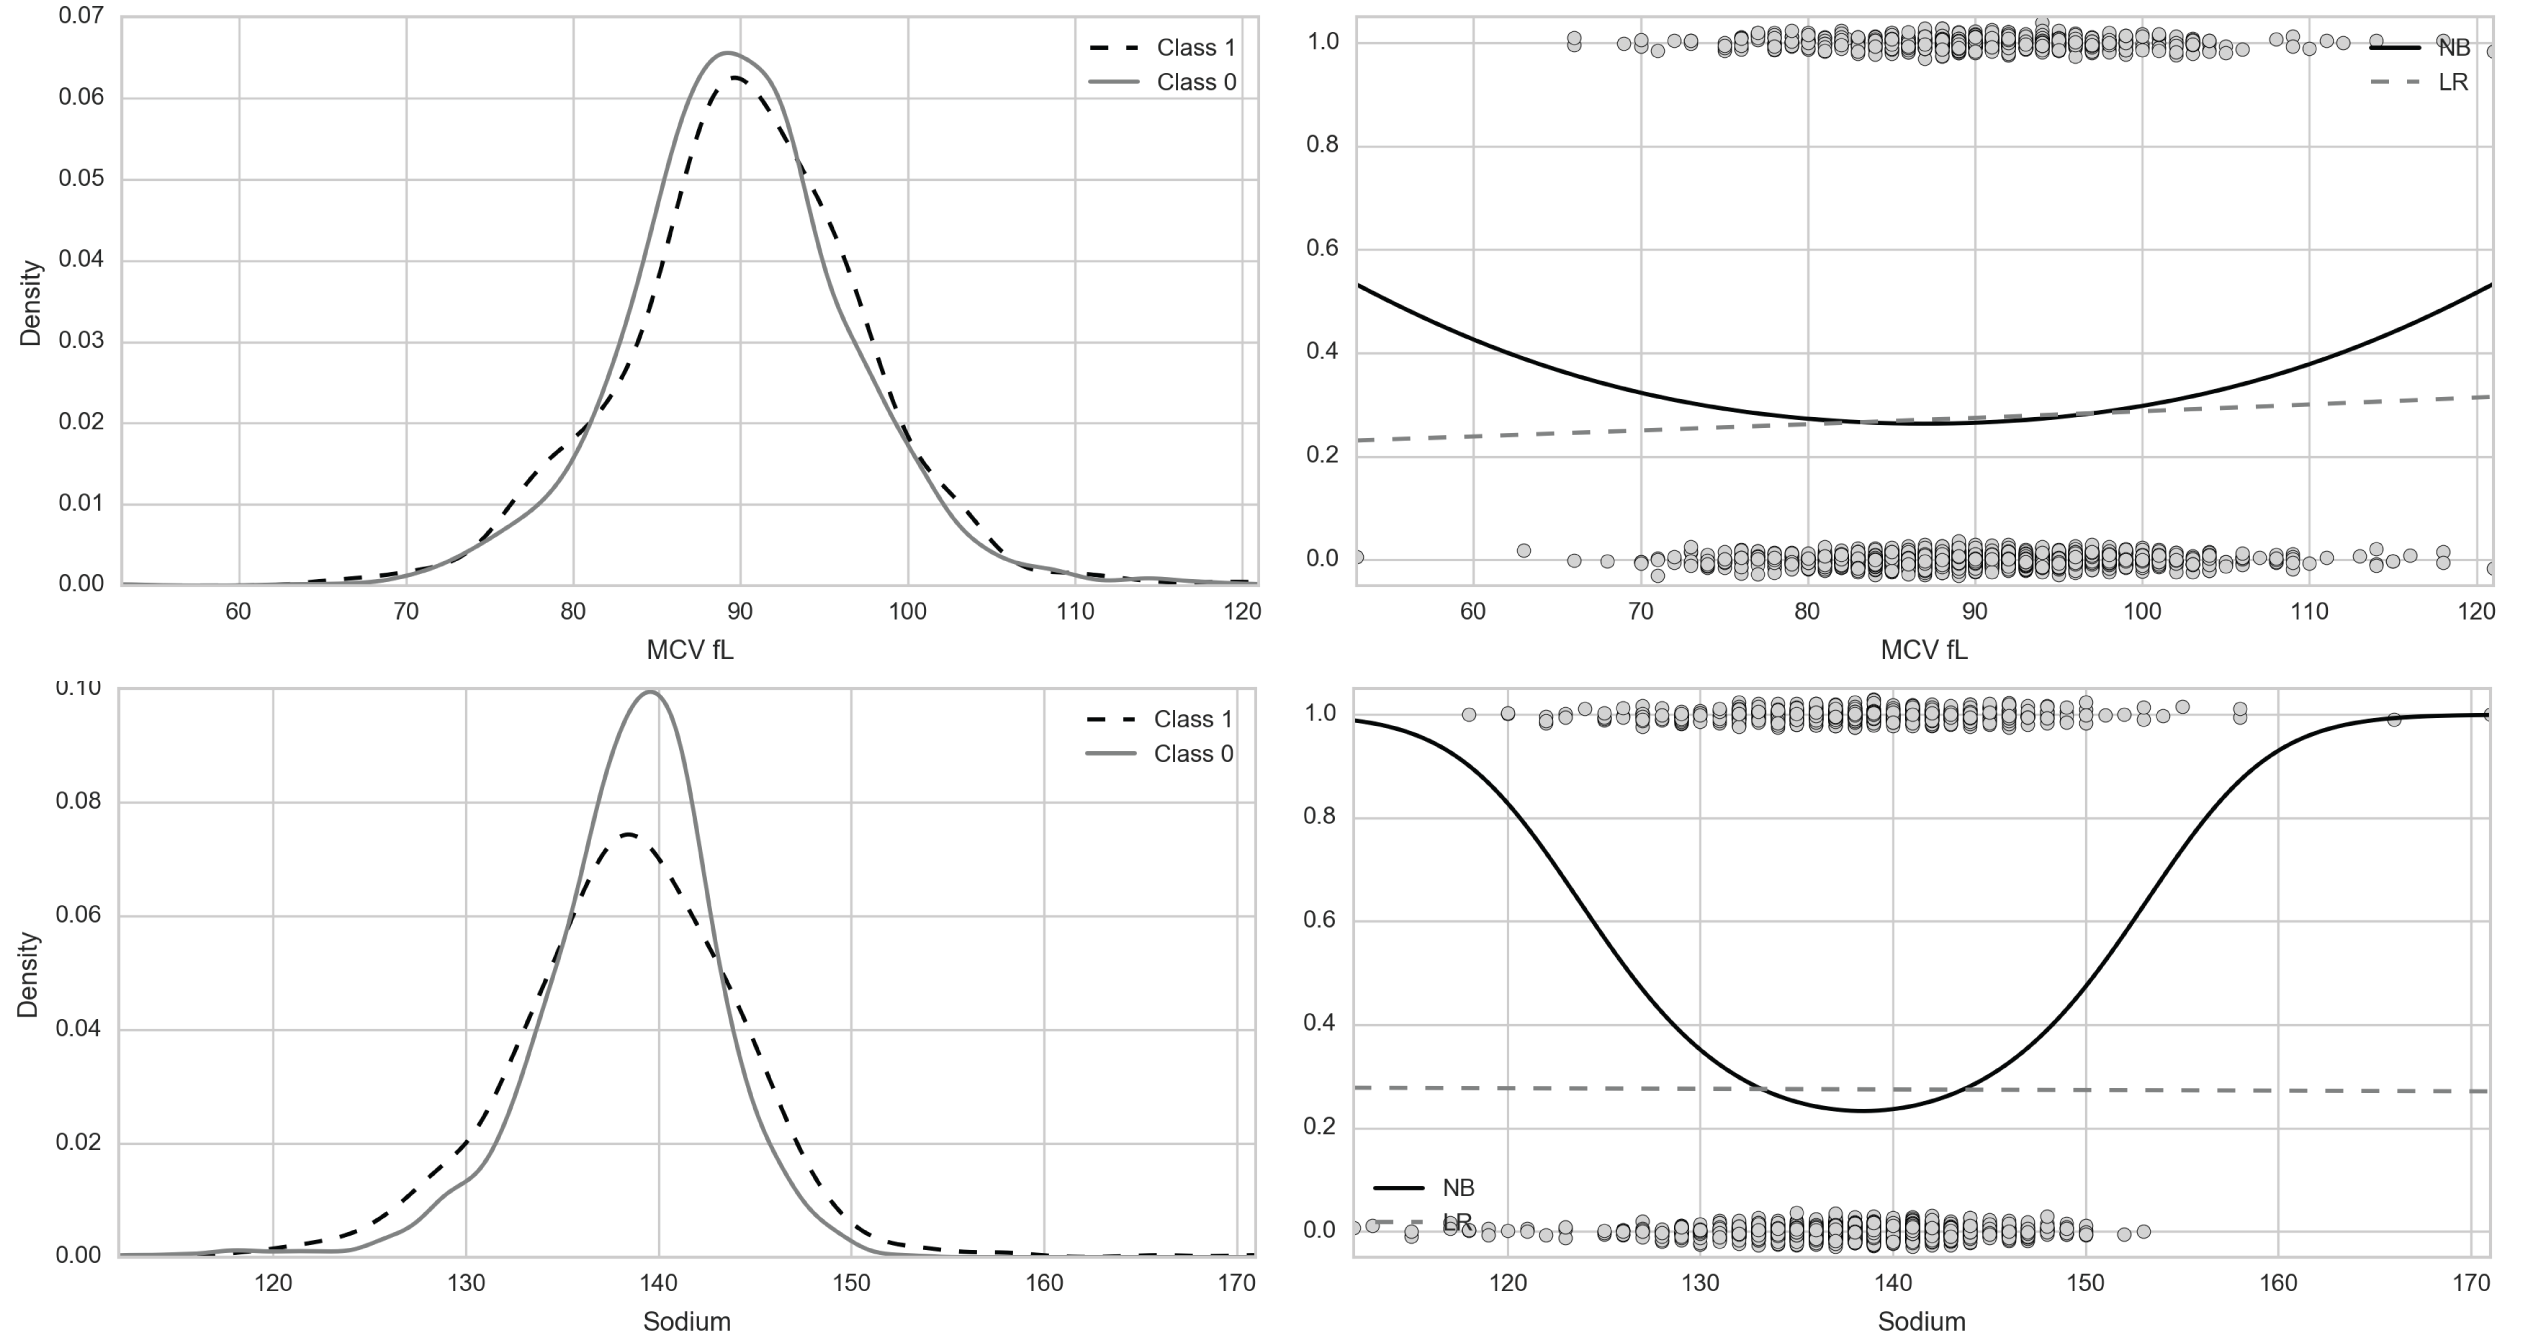
\includegraphics[width=\textwidth]{MCV_Sodium.png}
\caption{Density plots for both classes (left) and predictive model estimations (right) for MCV and Sodium.}
\label{fig:sodium}
\end{figure}

\begin{figure}[h!]
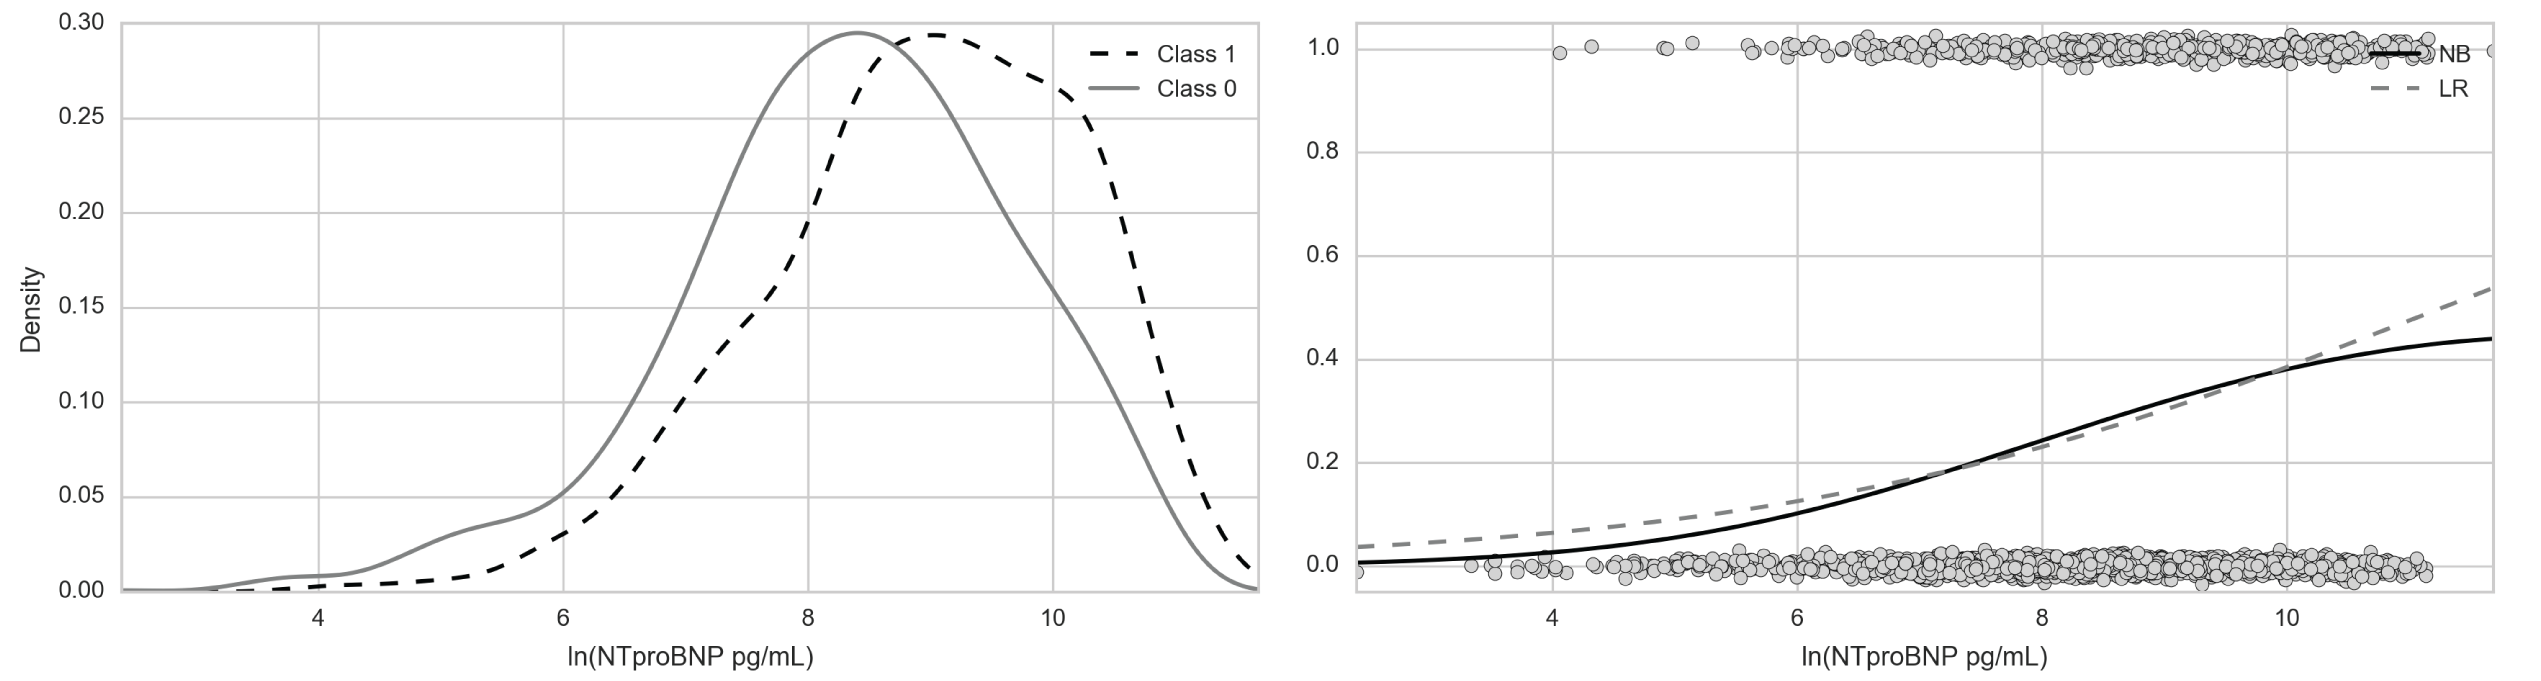
\includegraphics[width=\textwidth]{NTproBNP-01.png}
\caption{Density plots for both classes (left) and predictive model estimations (right) for NTproBNP.}
\label{fig:ntprobnp}
\end{figure}

The plots for NTproBNP which has been transformed using a natural logarithm where it can be seen that the estimates from logistic regression and naïve Bayes are similar (Figure \ref{fig:ntprobnp}).



\subsection*{Clinical Ranges}

To further explore the accuracy of the models at determining risk, three ranges (low, medium, high) where selected from each variable. The proportion of mortality events are calculated within these ranges and formed the ground truth for comparison. Risk estimations for both models are recorded on the original data and log transformed data. 

The results for these tests show that overall the naïve Bayes model gave a closer estimate of risk to the ground truth values (Table \ref{table:riskestimates}). The distribution of Creatinine is positively skewed with logistic regression giving more accurate estimation. However, when the variable is transformed to a natural logarithm scale the naïve Bayes provides closer estimations. For values greater than 8 mg/dL, the naïve Bayes model gives a better representation of risk.

In variables where the data is closer to being normally distributed such as Potassium and Sodium it can be seen that the naïve Bayes model gives better estimations (Table \ref{table:riskestimates}). This is true for both the original data and the log transformed data where estimations from a naïve Bayes model are closer to the true values than estimates from the logistic regression model.


\begin{table}[h]
\centering
\caption{Estimation Accuracy using a sample of ranges}
\label{table:riskestimates}
\begin{tabular}{lll|ll|ll}
\hline
\textbf{}         & \textbf{}       & \textbf{}   & \multicolumn{2}{c|}{\textbf{Raw}} & \multicolumn{2}{c}{\textbf{Log}} \\
\textbf{Variable} & \textbf{Range}  & \textbf{True \%} & \textbf{LR}     & \textbf{NB}    & \textbf{LR}     & \textbf{NB}    \\
\hline
Creatinine & 1 - 1.2         & 0.211 & 0.268      & 0.294      & 0.264      & 0.261      \\
Creatinine & 4 - 4.5         & 0.346 & 0.302      & 0.208      & 0.324      & 0.334      \\
Creatinine & 08 - 12         & 0.077 & 0.368      & 0.002      & 0.365      & 0.409      \\
Glucose    & 50 - 60         & 0.375 & 0.282      & 0.267      & 0.286      & 0.292      \\
Glucose    & 190 - 200       & 0.417 & 0.271      & 0.279      & 0.270      & 0.270      \\
Glucose    & 350 - 400       & 0.304 & 0.257      & 0.108      & 0.262      & 0.269      \\
NTproBNP   & 150 - 200       & 0.053 & 0.211      & 0.195      & 0.095      & 0.061      \\
NTproBNP   & 19,000 - 20,000 & 0.364 & 0.333      & 0.297      & 0.374      & 0.374      \\
NTproBNP   & 45,000 - 50,000 & 0.269 & 0.552      & 0.927      & 0.454      & 0.415      \\
Potassium  & 3 - 3.2         & 0.360 & 0.259      & 0.292      & 0.260      & 0.309      \\
Potassium  & 4.8 - 5         & 0.234 & 0.282      & 0.268      & 0.281      & 0.234      \\
Potassium  & 9 - 10          & 0.714 & 0.349      & 0.987      & 0.314      & 0.770      \\
Sodium     & 125 - 128       & 0.464 & 0.276      & 0.494      & 0.280      & 0.494      \\
Sodium     & 138 - 140       & 0.242 & 0.275      & 0.234      & 0.275      & 0.237      \\
Sodium     & 150 -155        & 0.714 & 0.273      & 0.604      & 0.269      & 0.536      \\
\hline
\end{tabular}
\end{table}


\subsection*{Metrics}
Whilst it is expected that the results using Pseudo R2, MSE and AUC will be poor for a single variable, the results have been shown to explore measurable differences in the models performance.

When comparing pseudo R2 and MSE there is subtle differences between the two models for all clinical variables (Table \ref{table:results1}). With variables such as Creatinine and NTproBNP which are highly skewed it is shown that logistic regression has a better AUC. However, when these variables are transformed using the natural logarithm (ln) the AUC is the same for both models. In contrast, naïve Bayes performs better with variables which are approximately normally distributed as shown with MCV and Sodium.

\begin{table}[h]
\centering
\caption{Results comparing psuedo $R^2$, Mean Square Error (MSE) and Area under the Curve (AUC)}
\label{table:results1}
\begin{tabular}{llll|lll}
\hline
\textbf{}            & \multicolumn{3}{c|}{\textbf{Naïve Bayes}}  & \multicolumn{3}{l}{\textbf{Logistic Regression}} \\

\textbf{Variable}    & \textbf{R2} & \textbf{MSE} & \textbf{AUC} & \textbf{R2}    & \textbf{MSE}    & \textbf{AUC}   \\
\hline
Creatinine mg/dL     & -0.006    & 0.200      & 0.515    & 0.001       & 0.199       & 0.547       \\
ln(Creatinine mg/dL) & 0.002     & 0.199    & 0.547    & 0.003       & 0.199       & 0.547       \\
MCV fL               & 0.000     & 0.199    & 0.534    & 0.000           & 0.199       & 0.519       \\
ln(MCV fL)           & 0.000     & 0.199    & 0.532    & 0.000           & 0.199       & 0.519       \\
NTproBNP pg/mL       & -0.025    & 0.204    & 0.624    & 0.036       & 0.192       & 0.633       \\
ln(NTproBNP pg/mL)   & 0.040      & 0.191    & 0.633    & 0.044       & 0.191       & 0.633       \\
Glucose mg/dL        & -0.004    & 0.200     & 0.500      & 0.000           & 0.199       & 0.495       \\
ln(Glucose mg/dL)    & 0.000      & 0.199    & 0.494    & 0.000           & 0.199       & 0.495       \\
Bicarbonate          & 0.007     & 0.198    & 0.551    & 0.003       & 0.199       & 0.538       \\
ln(Bicarbonate)      & 0.004     & 0.198    & 0.552    & 0.005       & 0.198       & 0.538       \\
Potassium            & -0.019    & 0.203    & 0.535    & 0.001       & 0.199       & 0.508       \\
ln(Potassium)        & -0.003    & 0.200      & 0.535  & 0.000     & 0.199       & 0.508       \\
Sodium               & 0.004     & 0.198    & 0.573    & 0.000           & 0.199       & 0.508       \\
ln(Sodium)           & 0.003     & 0.199    & 0.572    & 0.000           & 0.199       & 0.508       \\
\hline
\end{tabular}
\end{table}


\section{Discussion}

Discriminative models estimate the model parameters based on separation by minimising the negative log-likelihood classification loss against the true density [15]. Due to the nature of how the model parameters are estimated these types of models are regarded as supervised learning [16]. Discriminative models can be susceptible to cost or class imbalances in real world scenarios and in instances where the negative examples are more prevalent they are known to over fit [17]. This class imbalance problem is common in clinical datasets when developing models to predict mortality events [18]. 

The key feature of generative models is that the probability estimates of $p(y|x)$ are derived from the parameters of $p(x|y)$ and $p(x)$ which are estimated directly from the data. This involves internally representing the distribution of the data which adds an extra step in the probability estimations process. In the case of the naïve Bayes model $p(x|y)$ and $p(x)$ are assumed to be normally distributed, however, as shown, this is rarely the case with clinical data. Therefore, the application of generative models can be said to be more complex and it is recommended that you should not solve a more difficult problem as an intermediate step [19]. However by modelling the distribution of the input this information is incorporated into the model [16].

When comparing logistic regression and naïve Bayes it is concluded that discriminative models will perform better than generative models when considering the asymptotic errors [1]. However it has been shown that with real world datasets this may not always be the case [20]. When applying the two models to real clinical data it is shown that logistic regression models performed better when the data is highly skewed. Discriminative models learn the model parameters from maximizing the conditional likelihood [20] therefore, with skewed data the model estimations will be skewed towards the higher density regions of the variables distributions. Once the distributions are closer to been normally distributed the estimations of naïve Bayes become more accurate and gives a better representation of the the relationship between the inputs and the class. This is especially true when the means for the class are similar but the shape of the distributions are dissimilar, as shown with MCV and Sodium. As the applied Gaussian naïve Bayes model takes its estimations from normal distributions based on the mean and standard deviation for each class it can more accurately estimate the relationship between the inputs and class when the data is normally distributed. In these cases, generative linear models can determine nonlinear relationships between the input variable and the class. In contrast the linear discriminative nature of logistic regression implies that the probability estimates must either increase monotonically, or decrease monotonically in relation to the input [21].

One of the key features of this work is the demonstration of generative and discriminative linear models on clinical data. While the use of linear discriminative models, specifically logistic regression, is favoured within the development of clinical risk models these models may not always be appropriate. This is shown when performing a univariate analysis on variables such as Sodium and MCV (Fig. 1). When looking at Sodium the results from the logistic regression model show no evidence that Sodium levels which are too high or too low have an impact on mortality, despite this relationship been known [14]. When looking at the probability estimations for Sodium using a naïve Bayes model it is shown that these estimates are similar to the ground truth (Table 2). This is a result of the two classes having similar means, however, class 1 (dead) has a greater proportion of the data points within the extremities of the distribution. This is similar to values reported in a study using a heart failure dataset when looking at the means for Sodium of the two groups of patients. It is shown that alive patients had a mean Sodium level of 138.93 and those who died had a mean of 138.45, with differences in the standard deviations, 3.00 and 3.56 respectively [18].


\section{Conclusion}
In this study discriminative and generative models have been applied to clinical data with the results showing that both models perform equally well in scenarios where the classes are linearly separable. It is shown that the generative model of naïve Bayes is better at modelling the relationship between the input variable and class label when distributions for each class is not linearly separable. When applying this to clinical data it is shown that when using naïve Bayes as a generative model, the assumption of the input variables been normally distributed is important. In variables which are not separable and normally distributed the generative model gave more accurate estimations compared to the ground truth. The work concludes that the choice of discriminative and generative models is related to the data and dependant on the task which is to be modelled.

This work forms the foundation for model selection within a clinical dataset and future work should explore the comparison of discriminative and generative models in a multivariate context using clinical data. This should include the use of non-linear discriminative models such as SVMs and MLPs.


%%
%% Bibliography
%%

%% Either use bibtex (recommended), 

\bibliography{oasics-v2016-sample-article}

%% .. or use the thebibliography environment explicitely
[1]	A. Y. Ng and M. I. Jordan, “On Discriminative vs. Generative classifiers: A comparison of logistic regression and naive Bayes,” Adv. Neural Inf. Process. Syst., vol. 2, pp. 841–848, 2002.

[2]	J. J. G. G.-J. De Vries, G. Geleijnse, A. Tesanovic, and  a. R. T. R. Van De Ven, “Heart Failure Risk Models and Their Readiness for Clinical Practice,” 2013 IEEE Int. Conf. Healthc. Informatics, pp. 239–247, 2013.

[3]	R. Amarasingham, B. J. Moore, Y. P. Tabak, M. H. Drazner, C. A. Clark, S. Zhang, W. G. Reed, T. S. Swanson, Y. Ma, and E. A. Halm, “An Automated Model to Identify Heart Failure Patients at Risk for 30-Day Readmission or Death Using Electronic Medical Record Data,” Med. Care, vol. 48, no. 11, p. 981, 2010.

[4]	G. M. Felker, J. D. Leimberger, R. M. Califf, M. S. Cuffe, B. M. Massie, K. F. Adams, M. Gheorghiade, and C. M. O’Connor, “Risk stratification after hospitalization for decompensated heart failure,” J. Card. Fail., vol. 10, no. 6, pp. 460–466, 2004.

[5]	P. W. Wilson, R. B. D’Agostino, D. Levy, A. M. Belanger, H. Silbershatz, and W. B. Kannel, “Prediction of coronary heart disease using risk factor categories.,” Circulation, vol. 97, no. 18, pp. 1837–1847, 1998.

[6]	S. J. Pocock, C. A. Ariti, J. J. V McMurray, A. Maggioni, L. Køber, I. B. Squire, K. Swedberg, J. Dobson, K. K. Poppe, G. a. Whalley, and R. N. Doughty, “Predicting survival in heart failure: A risk score based on 39 372 patients from 30 studies,” Eur. Heart J., vol. 34, no. 19, pp. 1404–1413, 2013.

[7]	W. C. Levy, D. Mozaffarian, D. T. Linker, S. C. Sutradhar, S. D. Anker, A. B. Cropp, I. Anand, A. Maggioni, P. Burton, M. D. Sullivan, B. Pitt, P. A. Poole-Wilson, D. L. Mann, and M. Packer, “The Seattle Heart Failure Model: Prediction of survival in heart failure,” Circulation, vol. 113, no. 11, pp. 1424–1433, 2006.

[8]	E. W. Steyerberg, Clinical Prediction Models. Springer, 2009.

[9]	R. Alizadehsani, M. J. Hosseini, Z. A. Sani, A. Ghandeharioun, and R. Boghrati, “Diagnosis of Coronary Artery Disease Using Cost-Sensitive Algorithms,” 2012 IEEE 12th Int. Conf. Data Min. Work., pp. 9–16, 2012.

[10]	S. Palaniappan and R. Awang, “Intelligent Heart Disease Prediction System Using Data Mining Techniques,” IEEE/ACS Int. Conf. Comput. Syst. Appl., pp. 108–115, 2008.

[11]	L. Moore, C. Kambhampati, and J. G. F. Cleland, “Classification of a real live Heart Failure clinical dataset- Is TAN Bayes better than other Bayes?,” no. 1, pp. 882–887, 2014.

[12]	A. E. W. Johnson, T. J. Pollard, L. Shen, L. H. Lehman, M. Feng, M. Ghassemi, B. Moody, P. Szolovits, L. Anthony Celi, and R. G. Mark, “MIMIC-III, a freely accessible critical care database,” Sci. Data, vol. 3, p. 160035, 2016.

[13]	NICE, “Chronic heart failure - Management of chronic heart failure in adults in primary and secondary care,” NICE Clin. Guidel., no. August 2010, 2010.

[14]	J. Bohacik, C. Kambhampati, D. N. Davis, and J. G. F. Cleland, “Prediction of mortality rates in heart failure patients with data mining methods,” Ann. UMCS, Inform., vol. 13, no. 2, pp. 7–16, 2013.

[15]	G. Bouchard and B. Triggs, “The Tradeoff Between Generative and Discriminative Classifier,” in 16th IASC International Symposium on Computational Statistics, 2004, pp. 721–728.

[16]	O. . Chapelle, B. Schölkopf, and A. Zien, Semi-Supervised Learning. London: MIT Press, 2006.

[17]	N. V Chawla, N. Japkowicz, and P. Drive, “Editorial: Special Issue on Learning from Imbalanced Data Sets,” ACM SIGKDD Explor. Newsl., vol. 6, no. 1, pp. 1–6, 2004.

[18]	L. Moore, “Data Mining for Heart Failure: An investigation into the challenges un real life clinical datasets,” University of Hull, 2015.

[19]	V. N. Vapnik, Statistical Learning Theory. Wiley-Interscience, 1998.

[20]	J. H. Xue and D. M. Titterington, “Comment on ‘on discriminative vs. generative classifiers: A comparison of logistic regression and naive bayes,’” Neural Process. Lett., vol. 28, no. 3, pp. 169–187, 2008.

[21]	C. Elkan, “Maximum Likelihood , Logistic Regression , and Stochastic Gradient Training,” Tutor. notes CIKM, p. 11, 2012.


\end{document}
